\section{Theorie}
\label{sec:Theorie}
Ziel des Versuches ist es, Leerlaufspannungen und Innenwiderstände verschiedener 
Spannungsquellen zu bestimmen.

Unter dem Begriff "Spannungsquelle" wird ein Gerät verstanden, dass über
einen endlichen Zeitraum konstante elektrische Leistung liefern kann. 
Beispiele sind Galvanische Elemente, Dynamos oder LC - Generatoren. 
Als Leerlaufspannung $U_0$ bezeichnet man diejenige Spannung, die anliegt,
wenn der Quelle kein Strom $I$ entnommen wird. 
Wird ein Verbraucher an die Quelle angeschlossen, sinkt die "Klemmspanung"
$U_k$ auf einem Wert unter $U_0$ ab. Es gilt also $U_k < U_0$. Dies kann man 
durch die Zuordnung eines Innenwiederstandes $R_i$ zu der Spannungsquelle 
erklären. 
Das Ersatzschaltbild einer realen Spannungsquelle ist in Abbildung 
1 in dem gestrichelten Bereich dargestellt. 

\begin{figure}
\center
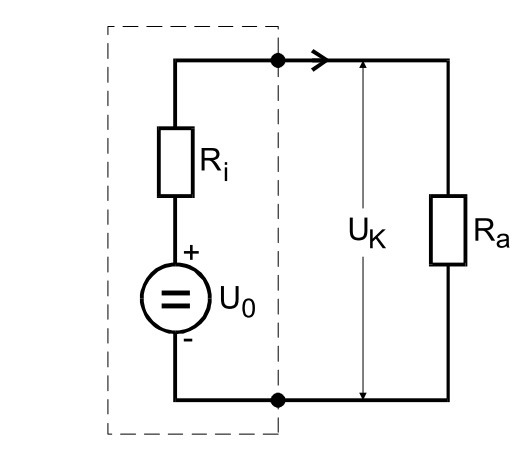
\includegraphics[scale=0.3]{Ersatzschaltbild.jpg}
\caption{Ersatzschaltbild für eine reale Spannungsquelle mit Lastwiderstand $R_a$}
\label{fig:Ersatz}
\end{figure}

Das Zweite Kirchhoffsche Gesetz, die Maschenregel, besagt, dass die Summe der 
Leerlaufspannungen gleich der Summe der Spannungsabfälle an den Widerständen der 
Masche ist. Angewandt auf unsere Schaltung ergibt sich:

\begin{equation}
U_k = I\cdot R_a = U_0 - I\cdot R_i
\label{eqn:Maschenregel}
\end{equation}

Daraus folgt direkt, dass $U_k$ mit zunehmdem Stromfluss abnehmen muss. 
Möchte man nun $U_0$ messen, ist es dementsprechend sinnvoll ein Spannungsmessgerät
mit hohem Innenwiderstand zu verwenden. Da $I=\frac{U}{R}$ gilt, wird durch einen
hohen Innenwiderstand der durch das Messgerät fließende Strom minimiert. Dadurch kann in 
(1) $I\cdot R_i$ vernachlässtig werden, sodass $U_0\approx U_k$ gilt.

$R_i$ sorgt außerdem dafür, dass der Spannungsquelle keine beliebig hohe
elektische Leistung entnommen werden kann. Das wird deutlich durch Betrachtung der
Leistung: 

\begin{equation}
P = I^2\cdot R_a
\label{eqn:Leistung}
\end{equation}

Durch Umformen von \eqref{eqn:Maschenregel} nach $I$ ergibt sich:

\begin{equation}
I = \frac{U_0}{R_a + R_i}
\label{eqn:Stromstärke}
\end{equation}

Einsetzen von \eqref{eqn:Stromstärke} in \eqref{eqn:Leistung} liefert:

\begin{equation}
P = \frac{U_0^2\cdot R_a}{(R_a + R_i)^2}
\label{eqn:Leistungsfunktion}
\end{equation}

Dies ist eine Funktion für die Leistung, die abhängig von $R_a$ ist. 
Untersucht man $P(R_a)$ genauer, so stellt man fest, dass die Funktion
ein Maximum durchläuft. Um festzustellen, an welcher Stelle dieses 
Maximum liegt, wird \eqref{eqn:Leistungsfunktion} zunächst abgeleitet.

\begin{equation}
\frac{\partial P}{\partial R_a} = \frac{U_0^2\cdot (R_i^2 - Ra^2)}{(R_a+R_i)^4}
\end{equation}

Das Maximum ergibt sich nun durch Nullsetzen der ermittelten Ableitung. 

\begin{align*}
&\quad \frac{\partial P}{\partial R_a} = 0 \\
&\Leftrightarrow U_0^2(R_i^2-R_a^2) = 0 \\
&\Leftrightarrow R_a = R_i 
\end{align*}

Der letzte Schritt ergibt sich, da $R_a, R_i > 0$ gilt. Das bedeutet, dass
die Leistung genau dann maximal wird, wenn der Innenwiderstand $R_i$ der 
Spannungsquelle genau dem Lastwiderstand $R_a$ entspricht. Diesen Fall
nennt man Leistungsanpassung. 

Auch Generatoren kann ein Innenwiderstand zugeordnet werden. Dieser muss
allerdings eine differentielle Größe 

\begin{equation}
R_i = \frac{\symup{d}U_k}{\symup{d} I}
\end{equation}

sein, da die Änderung des Belastungsstroms das elektrische Verhalten des 
Generators beeinflusst. 
